\documentclass[12pt]{report}
\usepackage{amsthm, amssymb}
\usepackage{geometry}
\geometry{legalpaper, margin=1in}
\usepackage{amsmath}
\usepackage{enumitem}

\newtheorem*{remark}{Remark}
\newtheorem{theorem}{Theorem}
\newtheorem{corollary}{Corollary}[theorem]
\newtheorem{lemma}[theorem]{Lemma}
\newtheorem*{defi}{Definition}
\newtheorem{ex}{Example}
\usepackage{xcolor}
\usepackage{graphicx}

\title{Topology HW 11}
\author{Ben Kallus}
\date{Due Monday, May 10, 2021}

\begin{document}
\maketitle

\medskip\noindent\textbf{1)} Proposition: $\mathbb R^n$ is simply connected.

    Let $n \geq 1$.
    Then, $\mathbb R^n = \mathbb R \times \hdots \times \mathbb R$.
    Let $f$ be a loop in $\mathbb R$ from $a$ to $b$ and back.
    Then, $f \in [e]$ because by smoothly sliding $b$ to $a$, $f$ can be continuously deformed into $e$.
    Thus, $\mathbb R$ is simply connected.
    Thus, by Theorem 52.023, $$\pi_1(\mathbb R^n) = \pi_1(\mathbb R \times \hdots \times \mathbb R) = \pi_1(\mathbb R) \times \hdots \times \pi_1(\mathbb R) = \{[e]\} \times \hdots \times \{[e]\} = \{[e]\}.$$
    Thus, $\mathbb R^n$ is simply connected.

\newpage\noindent\textbf{2)}

\medskip\noindent\textbf{(a)} Find a star convex set that is not convex.

Consider the following subset $A$ of $\mathbb R^2$, shown in blue in the picture below:
\begin{center} 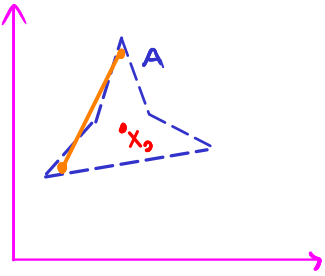
\includegraphics{1.png} \end{center}
$A$ is not convex because of the orange line segment.
$A$ is star convex because of the point $x_0$.

\medskip\noindent\textbf{(b)} Proposition: If $A$ is star convex, then $A$ is simply connected.
\begin{proof}
    Let $n \in \mathbb N$, and let $A \subseteq \mathbb R^n$ be star convex.
    Let $\mathbf x, \mathbf y \in \mathbb R^n$
    Then, there exists $a_0 \in A$ such that there is a line segment from $\mathbf x$ to $a_0$, and another line segment from $a_0$ to $\mathbf y$.
    Thus, $A$ is path connected, because following these line segments sequentially yields an $\mathbf x$ $\mathbf y$ path.
    Let $f$ be a loop in $A$ based at $a_0$.
    Then, $F: [0,1] \times [0,1] \to \mathbb A$ defined by $$F(s, t) = f(s)(1-t) + at$$ is a homotopy from $f$ to $e$.
    Note that each intermediate loop in this homotopy is fully contained in $A$, because every point in $A$ is visible from $a_0$.
    Thus, $\mathbb A$ is simply connected.
\end{proof}

\newpage\noindent\textbf{3)} Compute $\pi_1(S^1 \times S^1, x_0)$ and $\pi_1(S^1 \times [0,1],x_0)$.
\begin{proof}
    By Theorem 52.021, $\pi_1(S^1) \cong \mathbb Z$.
    Note that $S^1$ is path-connected because any pair of points on a circle can be joined by an arc.
    Thus, by Theorem 52.023, $\pi_1(S^1 \times S^1) \cong \pi_1(S^1) \times \pi_1(S^1) \cong \mathbb Z \times \mathbb Z$.

    Note that $[0,1]$ is path-connected because any two points $a,b \in [0,1]$ are connected by the path $f: [0,1] \to [0,1]$ defined by $f(t) = a(1-t)+bt$.
    Observe that the fundamental group of $[0,1]$ is the trivial group, because any loop from $a$ to $b$ and back can be continuously deformed into the identity loop by smoothly sliding $b$ to $a$.
    Thus, $\pi_1(S^1 \times [0,1]) \cong \pi_1(S^1) \times \pi_1([0,1]) \cong \mathbb Z \times \{[e]\} \cong \mathbb Z$.
\end{proof}

\end{document}
